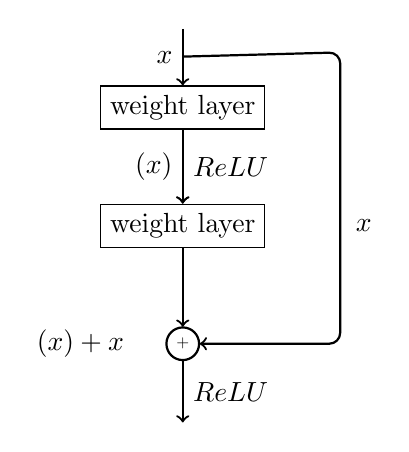
\begin{tikzpicture}
    
    \node[rectangle, draw] (n1) at (0,0) {weight layer};
    \node[rectangle, draw] (n2) at (0,-1.5) {weight layer};
    \node[circle, draw, scale =.6, thick] (n3) at (0,-3) {$\mathbf{+}$};
    
    \draw[thick, ->] (0,1) -- (n1) node[midway, left] (a1) {$x$};
    \draw[thick, ->] (n1) -- (n2) node[midway, left] {$\F (x)$} node[midway, right] {$ReLU$};
    \draw[thick, ->] (n2) -- (n3);
    
    \draw[thick, ->,rounded corners] (a1) -- node[]{} (2,.7) |- (n3);

    \draw[thick, ->] (n3) -- (0,-4) node[midway, right] {$ReLU$};
    
    \draw (-1.3,-3) node[] {$\F(x) + x$};
    \draw (2.3,-1.5) node[] {$x$};
    \draw[thick,->] (n1) -- (n2);
\end{tikzpicture}